\begin{figure}[tbp]
\centering
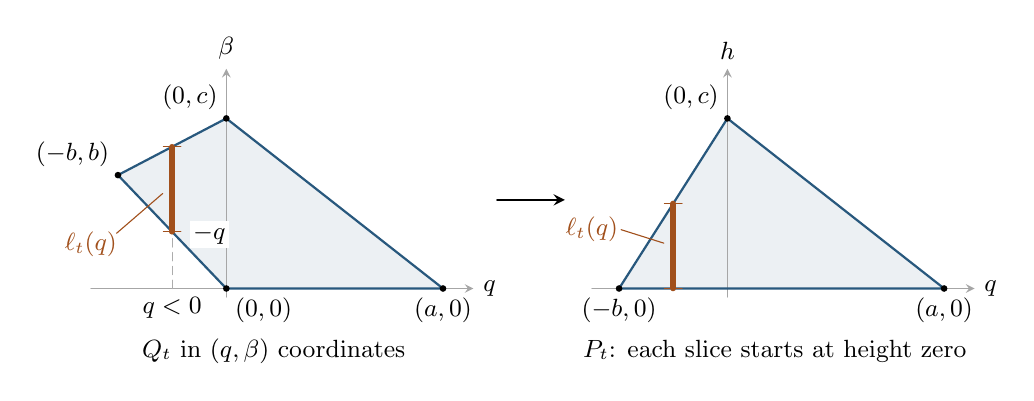
\begin{tikzpicture}[x=.86cm,y=.90cm,font=\small,
  line cap=round,line join=round,>=stealth]
  \definecolor{diagramblue}{RGB}{40,88,125}
  \definecolor{diagramorange}{RGB}{161,80,28}
  \begin{scope}
    \fill[diagramblue!9] (0,0)--(3.2,0)--(0,2.4)--(-1.6,1.6)--cycle;
    \draw[->,gray!70] (-2.0,0)--(3.65,0) node[right,text=black] {$q$};
    \draw[->,gray!70] (0,-.12)--(0,3.1) node[above,text=black] {$\beta$};
    \draw[diagramblue,thick] (0,0)--(3.2,0)--(0,2.4)--(-1.6,1.6)--cycle;
    \draw[densely dashed,gray!65] (-.8,0)--(-.8,.8);
    \draw[diagramorange,line width=2pt] (-.8,.8)--(-.8,2.0);
    \draw[diagramorange] (-.93,.8)--(-.67,.8) (-.93,2.0)--(-.67,2.0);
    \node[diagramorange] at (-2.0,.62) {$\ell_t(q)$};
    \draw[diagramorange,thin] (-1.62,.78)--(-.94,1.34);
    \node[anchor=west,fill=white,inner sep=1.3pt] at (-.55,.76) {$-q$};
    \fill (0,0) circle (1.2pt) (3.2,0) circle (1.2pt)
          (0,2.4) circle (1.2pt) (-1.6,1.6) circle (1.2pt);
    \node[below right,inner sep=3pt] at (0,0) {$(0,0)$};
    \node[below,inner sep=3pt] at (3.2,0) {$(a,0)$};
    \node[above left,inner sep=3pt] at (0,2.4) {$(0,c)$};
    \node[above left,inner sep=3pt] at (-1.6,1.6) {$(-b,b)$};
    \node[below,inner sep=3pt] at (-.8,0) {$q<0$};
    \node[align=center] at (.7,-.88) {$Q_t$ in $(q,\beta)$ coordinates};
  \end{scope}
  \draw[->,thick] (4.0,1.25)--(5.0,1.25);
  \begin{scope}[shift={(7.4,0)}]
    \fill[diagramblue!9] (-1.6,0)--(3.2,0)--(0,2.4)--cycle;
    \draw[->,gray!70] (-2.0,0)--(3.65,0) node[right,text=black] {$q$};
    \draw[->,gray!70] (0,-.12)--(0,3.1) node[above,text=black] {$h$};
    \draw[diagramblue,thick] (-1.6,0)--(3.2,0)--(0,2.4)--cycle;
    \draw[diagramorange,line width=2pt] (-.8,0)--(-.8,1.2);
    \draw[diagramorange] (-.93,0)--(-.67,0) (-.93,1.2)--(-.67,1.2);
    \node[diagramorange] at (-2.0,.83) {$\ell_t(q)$};
    \draw[diagramorange,thin] (-1.57,.83)--(-.94,.64);
    \fill (-1.6,0) circle (1.2pt) (3.2,0) circle (1.2pt)
          (0,2.4) circle (1.2pt);
    \node[below,inner sep=3pt] at (-1.6,0) {$(-b,0)$};
    \node[below,inner sep=3pt] at (3.2,0) {$(a,0)$};
    \node[above left,inner sep=3pt] at (0,2.4) {$(0,c)$};
    \node[align=center] at (.7,-.88) {$P_t$: each slice starts at height zero};
  \end{scope}
\end{tikzpicture}
\caption{Diagonal compression of exponent slices. For $c(a+b)>ab$, the
change $q=\alpha-\beta$ turns $Q_t$ into the quadrilateral on the left.
Moving each vertical slice down to height zero gives $P_t$, with the
same slice length $\ell_t(q)$. The highlighted slice has $q<0$ and lower
endpoint $-q$. This diagram describes the containing regions; the jet
transfer is proved by convergence of finite jet matrices.}
\label{fig:compression}
\end{figure}
